% Gemini theme
% See: https://rev.cs.uchicago.edu/k4rtik/gemini-uccs
% A fork of https://github.com/anishathalye/gemini

\documentclass[final,20pt]{beamer}

% ====================
% Packages
% ====================
\usepackage{amsfonts}
\usepackage[T1]{fontenc}
\usepackage{lmodern}
\usepackage[size=A0,orientation=landscape,scale=1.2]{beamerposter}
\usetheme{gemini}
\usecolortheme{lsu}
\usepackage{xcolor}
\usepackage{graphicx}
\usepackage{booktabs}
\usepackage{siunitx}
\usepackage[flushleft]{threeparttable}
\usepackage{tikz}
\usepackage{pgfplots}
\usepackage{caption}
\usepackage{subcaption}
\pgfplotsset{compat=1.17}
\sisetup{uncertainty-mode = compact}
\sisetup{
	input-open-uncertainty=(,
	input-close-uncertainty=),
	output-open-uncertainty = (,
	output-close-uncertainty = ),
	uncertainty-separator = \,
}%

% ====================
% Lengths
% ====================

% If you have N columns, choose \sepwidth and \colwidth such that
% (N+1)*\sepwidth + N*\colwidth = \paperwidth
\newlength{\sepwidth}
\newlength{\colwidth}
\newlength{\colwidthbig}
\newlength{\colwidthsmall}
\setlength{\sepwidth}{0.025\paperwidth}
\setlength{\colwidth}{0.3\paperwidth}
\setlength{\colwidthbig}{0.38\paperwidth}
\setlength{\colwidthsmall}{0.26\paperwidth}

\newcommand{\separatorcolumn}{\begin{column}{\sepwidth}\end{column}}

% ====================
% Title
% ====================

\title{Are representations in the hippocampus\\organized by the emotional content of stimuli? \\ A multivariate analysis of intracranial electrode recordings}

\author{Alexander N. Lawriw \& Christopher R. Cox}
%\inst{1}
\institute[shortinst]{\textit{Louisiana State University, Baton Rouge, LA}}

% ====================
% Footer (optional)
% ====================

\footercontent{
  https://faculty.lsu.edu/chriscox \hfill
  Cognitive Neuroscience Society 2024, Toronto, CA \hfill
  \href{mailto:alawri1@lsu.edu}{alawri1@lsu.edu}}
% (can be left out to remove footer)

% ====================
% Logo (optional)
% ====================

% use this to include logos on the left and/or right side of the header:
\logoright{
\includegraphics[height=7cm]{figures/CoxHaebig2022_BRM_QRCode.png}}
\logoleft{
\includegraphics[height=7cm]{logos/LSU_Purple_CMYK.pdf}}

% ====================
% Body
% ====================

\begin{document}
%\addtobeamertemplate{headline}{}
%{
%    \begin{tikzpicture}[remember picture,overlay]
%      \node [anchor=north west, inner sep=3cm] at %([xshift=0.0cm,yshift=3cm]current page.north west)
%      {
\includegraphics[height=8.5cm]{logos/ucf_logo2.png}}; % also try %shield-white.eps
%      \node [anchor=north east, inner sep=3cm] at %([xshift=0.0cm,yshift=3cm]current page.north east)
%      {
\includegraphics[height=8.5cm]{logos/lab_logo.jpg}};
%    \end{tikzpicture}
%}

\begin{frame}[t]
\begin{columns}[t]
\separatorcolumn

\begin{column}{\colwidthsmall}

  \begin{block}{Introduction}

    \begin{itemize}
      \item Traditional views of the hippocampus highlight the region's role as a rapid encoder of episodic events \cite{mcclelland_why_1995}
      \item Recent work suggests the hippocampus may also be capable of representing learned structure, such as categorical information \cite{schapiro_human_2018}
      \item Emotional information appears to receive preferential processing in the hippocampus as evidenced by stronger memory for such stimuli \cite{dolcos_interaction_2004}
      \item Connected structures may provide 'emotional labels' to the hippocampus for use during encoding \cite{rolls_hippocampus_2022} 
      
    \end{itemize}
  \end{block}



  \begin{block}{Stimuli and Procedures}
      
    \begin{itemize}
        \item 120 computer-generated male faces six times each (720 trials).
        \item Morphed to convey positive, negative, or neutral affect (40 each).
        \item Participants view face  1 s, then report affect of facial expression.
    \end{itemize}
    
    \begin{figure}
        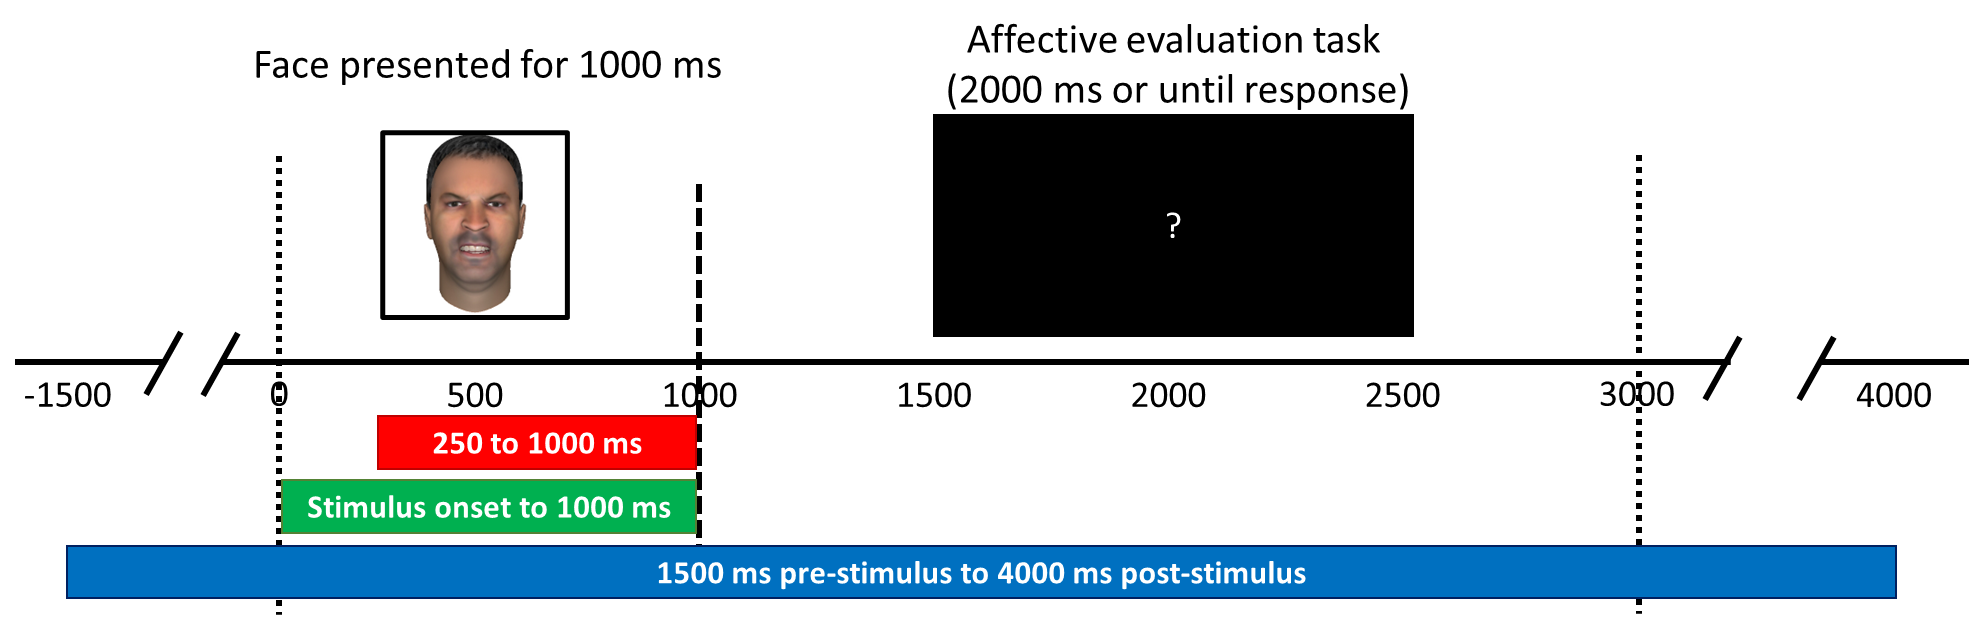
\includegraphics[width=1\textwidth]{figures/trial.png}
        \caption{Trial schematic. Time points contributing to spiking analysis (red), wavelet convolution (blue), and LFP analysis (green) are shown.
        }
    \end{figure}
            
  \end{block}

    \begin{block}{Recording Protocol}
  
   \begin{itemize}
        \item Microwires were implanted into the amygdala (AMG), hippocampus (HPC), ventromedial prefrontal cortex (vmPFC), and anterior cingulate cortex (ACC).
        \item HPC target was ``mid-body'' ($\sim$ CA3).
        \item 8 channels per brain region per hemisphere (64 channels total). 
        \item One set of decoding models were fit to single- and multi-unit spiking activity
        \item Second set of decoding models were fit to spectral power of LFPs (obtained via Morlet wavelet). 
   \end{itemize}
   
    \begin{figure}
        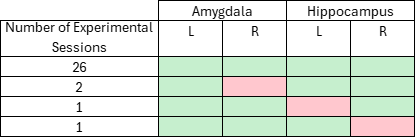
\includegraphics[width=.9\textwidth]{figures/recording sites.png}
        \caption{Presence (green) or absence (red) of electrodes in key brain regions.}
    \end{figure}
  \end{block}

 

\end{column}
\separatorcolumn

\begin{column}{\colwidthbig}
\begin{alertblock}{Research Questions}
    \centering
    \begin{itemize}
    	\item \textbf{Is affective information represented in the hippocampus?}
    	\item \textbf{If so, is this information represented in the spiking activity of individual neurons or in the local field potentials produced by much broader neuronal populations?}
    \end{itemize}
  \end{alertblock}
  \begin{block}{Theoretical Viewpoints}
    \begin{figure}
    \centering
    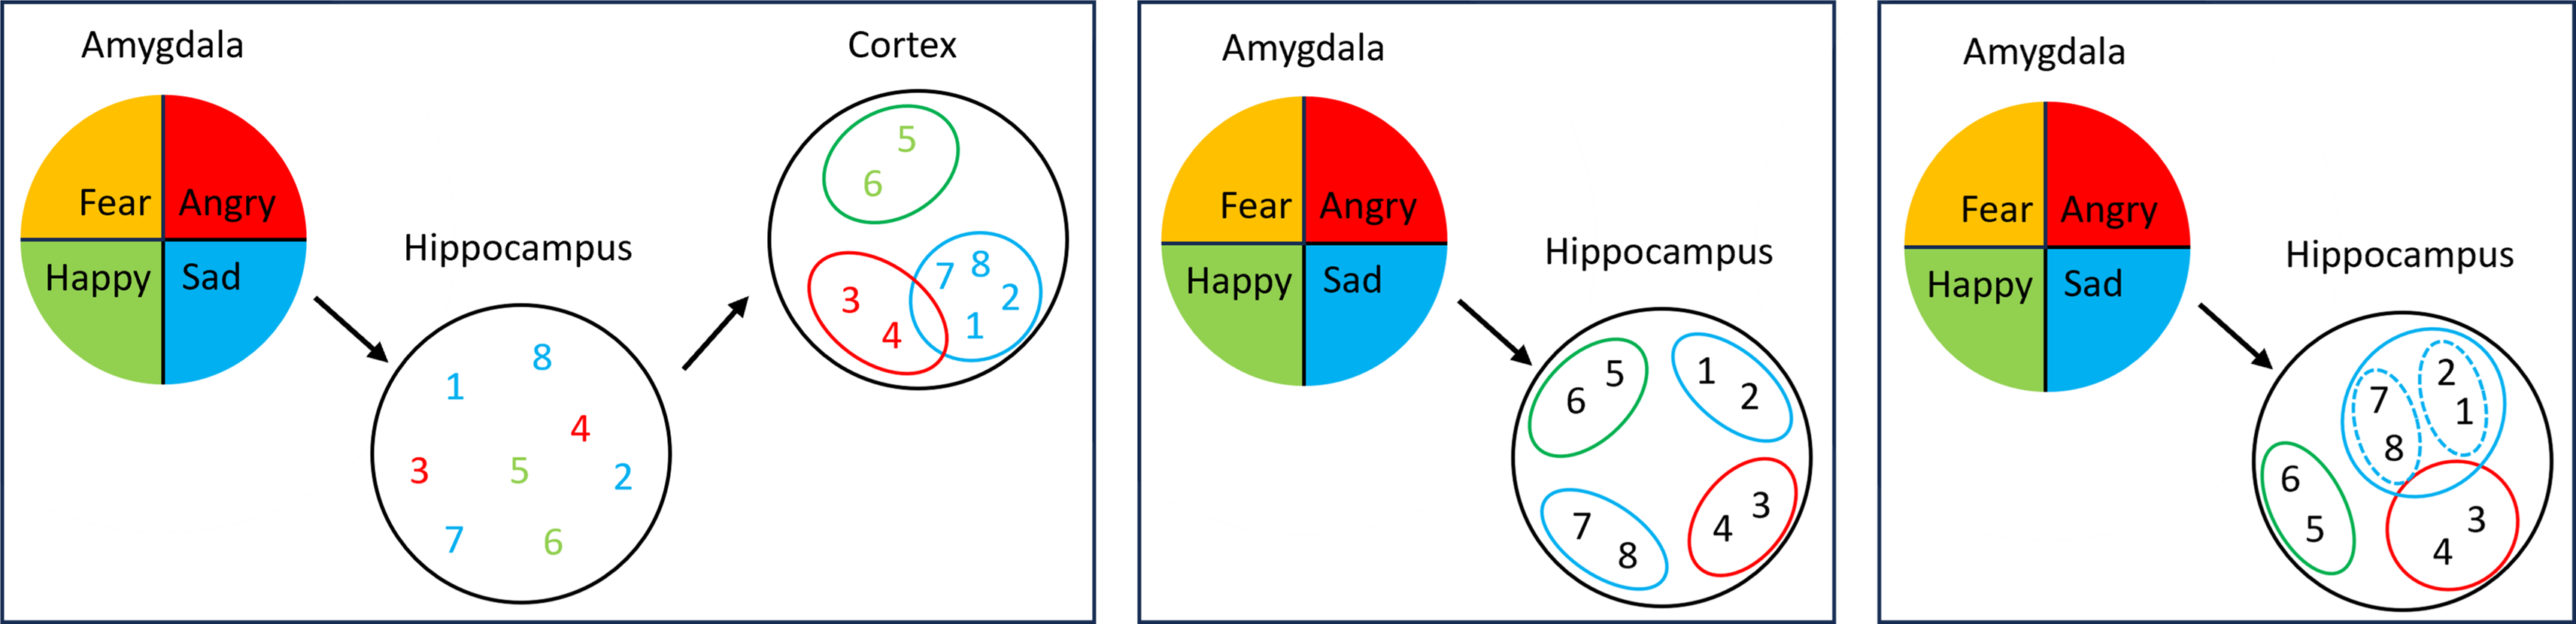
\includegraphics[width=1\textwidth]{figures/Theories.png}
    \caption{Different theoretical viewpoints on the role of the hippocampus in emotional memory. Left – emotional events are sparsely encoded in the hippocampus. Events similar in emotional content are represented similarly in the cortex. Middle – emotional information is used to group events that frequently co-occur together. Distinct temporal groupings are kept separate from one another. Right - Events similar in emotional content are represented using similar neural activity.}
    \end{figure}
  \end{block}

  \begin{block}{Accuracy of Cross-Validated Models}
    \begin{figure}
    \centering
     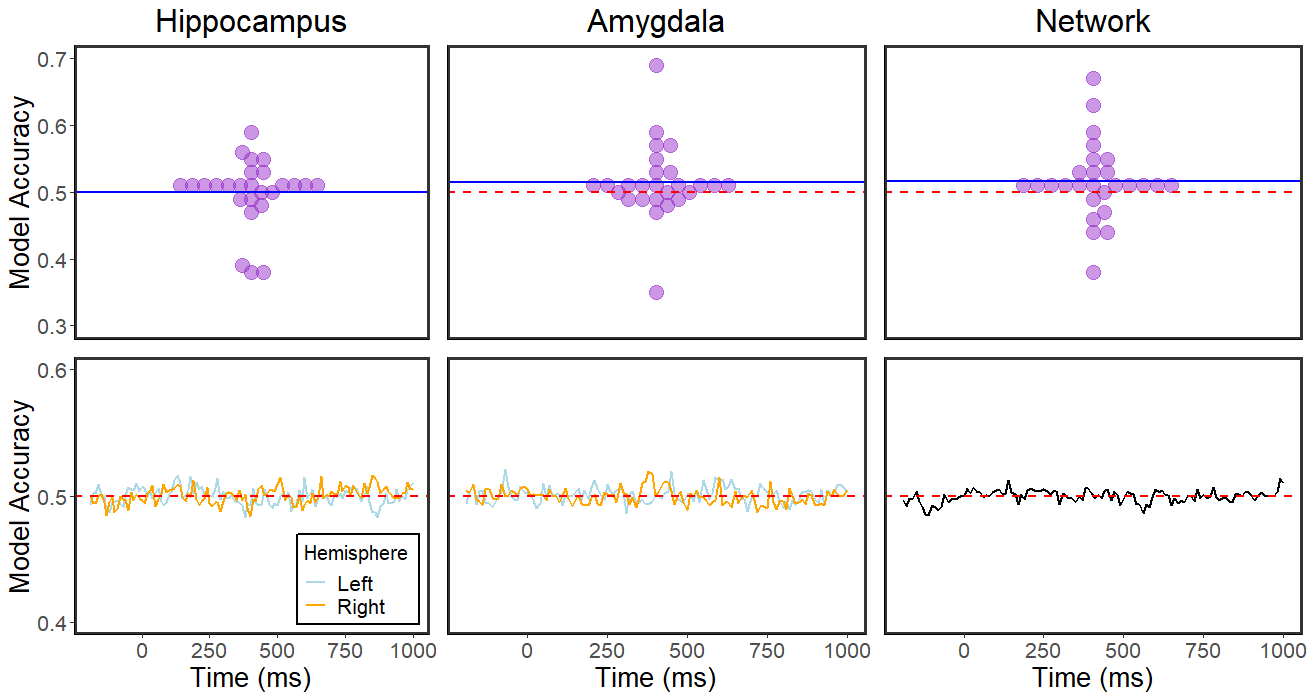
\includegraphics[width=1\textwidth]{figures/cns fig.png}
     \hfill
     \caption{Cross-validated accuracies of models built using spike counts (top row) or spectral power from LFPs (bottom row). Red line indicates chance level performance.}
    \end{figure}
  
%    \begin{figure}
%    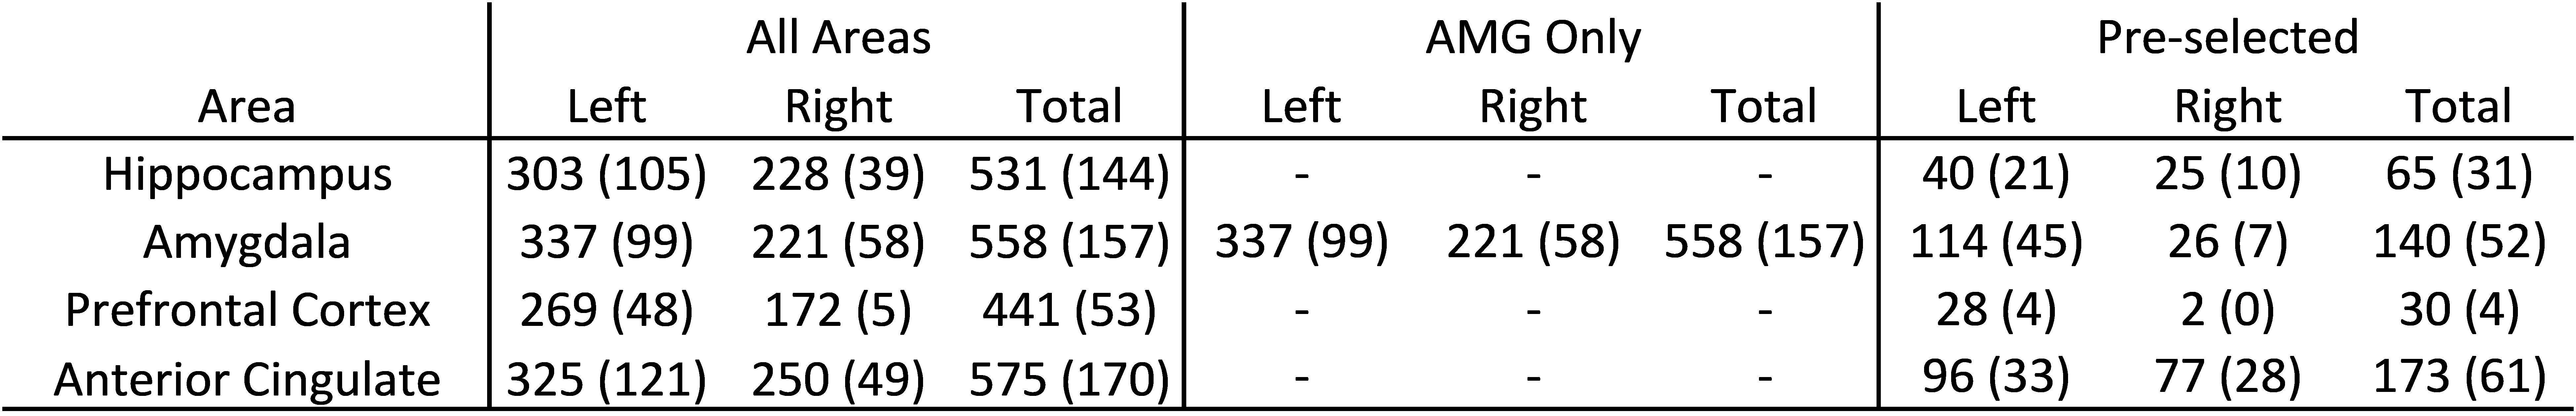
\includegraphics[width=.8\textwidth]{figures/ModelClusterCount.jpg}
%    \caption{Counts aggregate all 28 experimental sessions for the full and pre-selected models, and 26 sessions for the amygdala only models. Primary counts include single-unit activity (SUA) and multi-unit activity (MUA); counts in parenthesis reflect SUA.}
%    \end{figure}
    
    
  \end{block}

\end{column}

\separatorcolumn

\begin{column}{\colwidthsmall}

  \begin{block}{Participants}
    
    \begin{itemize}
        \item 30 experimental sessions from 14 pharmaco-resistant epilepsy patients (8 female; 20 -- 56 years; mean age = 40 years; 1 left handed). 
        \item Monitored for possible resection of an epileptogenic focus.
        \item 11 had seizure foci in hippocampus (5 L), 8 in amygdala (4 L, 1 B). 
    \end{itemize}
    

  \end{block}

  \begin{block}{Conclusions and Discussion}
    
    \begin{itemize}
        \item Unable to discriminate between positive and negative affect by modeling spike rates or time-varying LFP spectral power.
        %\item Our results do not support the existence of "affect detectors" in the limbic system and instead suggest a more complex representation of affect.
        \item Most consistent with sparse episodic encoding of individual faces.
        \item But results may be influenced by HPC implantation target $\sim CA3$.
        \item Cannot reject hypothesis that HPC represents categorical information while learning, before cortical consolidation.  
    \end{itemize}
    \begin{figure}
    \centering
    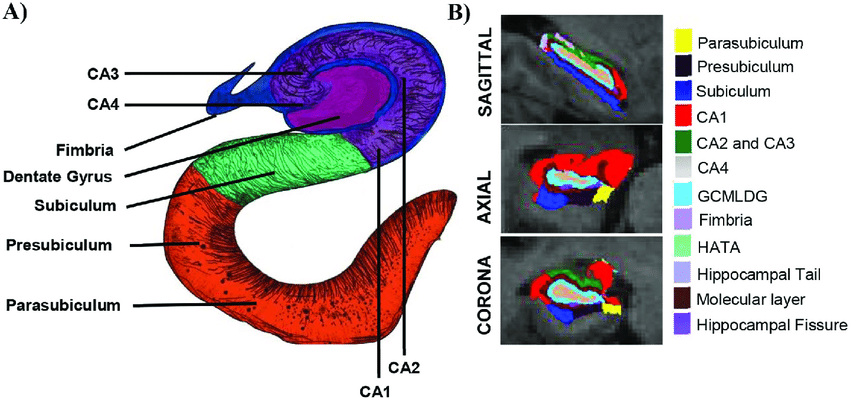
\includegraphics[width=.9\textwidth]{figures/Hippocampus subfields 3.png}
    \caption{Segmentation of human hippocampus into subfields.  Figure from Kannappan et al., 2022. \cite{kannappan_polygenic_2022} Published in the Public Library of Science under a CC Attribution License.  
    }
    \end{figure}
    

  \end{block}
  
  \begin{block}{Acknowledgments}
    
    \begin{itemize}
      \item We would like to thank Dr. Peter N. Steinmetz and the Neurtex Brain Research Institute for providing the data set and continued support.
    \end{itemize}
 
  \end{block}

  \begin{block}{References}

%    \nocite{*}
    \footnotesize{\bibliographystyle{ieeetr}\bibliography{CNS}}

  \end{block}
  

\end{column}

\separatorcolumn
\end{columns}
\end{frame}

\end{document}
